The set of all subsets of a finite set $A$ is called the powerset, $P(A)$, also written as $2^{A}$, because for every element $a \in A$ there are two possible outcomes, $a$ is in a subset or it isn't. Let $A$ be the set: $$A = \{ a_{1}, a_{2}, a_{3},..., a_{n}\},\ \lvert{A}\rvert = n$$
So starting with the empty set $\{ \}$ totaling $2^{0}$ subsets, for $a_{1} \rightarrow \{\}, \{a_{1}\}$ totaling $2\cdot2^{0} = 2^{1}$ and so on, until for $a_{n}$ the total number subsets is $2\cdot2^{n-1} =2^{n}$.
\bigskip

For Infinite sets and all arbitrary sets the powerset is always bigger than the set itself this can be proved with the same contradiction as in the real number proof above:
\bigskip

Let there be a complete list of all the subsets numerated by the members of the set, such that $\lvert{P(A)}\rvert = \lvert{A}\rvert$:

\begin{figure}[H]
    \centering
    \begin{minipage}{0.45\textwidth}
        \centering
        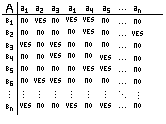
\includegraphics[width=\textwidth]{Illustrations/Powersets_no_diagonal.png}
        \label{fig:power_set1}
    \end{minipage}
    \hfill
    \begin{minipage}{0.45\textwidth}
        \centering
        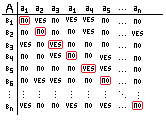
\includegraphics[width=\textwidth]{Illustrations/Powersets_with_diagonal.png}
        \label{fig:power_set2}
    \end{minipage}
    \caption{Arbitrary powerset and its 'complete' list}
\end{figure}

Forming this table of whether the element $a_{i} \in A$ is included in the subset $B_{i} \subset A$, we can again take a diagonal selection and invert the values, yes's to no's and vice versa. This creates a subset that is not included in the list of subsets, therefore it is not a complete list, and $\lvert{P(A)}\rvert > \lvert{A}\rvert$.
\bigskip

Therefore we can prove that the powerset of the natural  numbers is larger than the natural  numbers and uncountable.
\bigskip

If we attribute a code for the potential numbers and symbols appearing in every real number $[\text{'0'}:0,\text{'1'}:1,\text{'2'}:2,\text{'3'}:3,...,  ]$
If we attribute a code for the potential numbers and symbols appearing in every real number $$[\text{'0'}:0,\ \text{'1'}:1,\ \text{'2'}:2,\ \text{'3'}:3,\ ...\ ,\   \text{'9'}:9,\  \text{'-'}:10,\  \text{'.'}:11]$$ We can then maintain the order by adding a consecutive multiple of $100$ to each, so for example $12.5 \rightarrow \{1, 102,  211, 305\}$, or $-\sqrt{2} = \{10, 101, 211, 304,401, 502, ... \}$.
\bigskip

From this it is clear that, all Real numbers are contained within the powerset of the naturals, $\mathbb{R} \subset P(\mathbb{N})$, and $\lvert{P(\mathbb{N})}\rvert > \lvert{\mathbb{R}}\rvert$.

\begin{minipage}{0.2\textwidth}
    \includegraphics[width=\textwidth]{Illustrations/the_wiz_fails_to_argue.png}
\end{minipage}
\hfill
\begin{minipage}{0.75\textwidth}
    If you let each number represent a digit after the decimal in $0.$, then for all subsets $B \subset A, B \in P(A)$ they can be mapped to a real number between 0 and 1. So $P(A) \subset \mathbb{R}$.
\end{minipage}
\bigskip





